\chapter{Implementacja środowiska badawczego}
W niniejszym rozdziale przedstawiono proces implementacji środowiska badawczego pod kątem realizacji zdefiniowanych uprzednio scenariuszy badawczych. Spośród składowych omawianego procesu wyróznić należy: przygotowanie odmian topologii fizycznych środowiska w zależności od scenariusza badawczego, budowę interfejsów programowania aplikacji z wykorzystaniem porównywanych technologii, czy też zastosowanie mechanizmów pozwalających na weryfikację działania API w aspekcie programowania współbieżnego. Ponadto, zaprezentowana została konfiguracja dedykowanych porównywanym technologiom platform chmurowych, a także struktura elementów składających się na plan testowy, identyfikujący przeprowadzoną ewaluację w ramach narzędzia przeznaczonego do realizacji badań.    
\section{Realizacja topologii fizycznych}
W zależności od scenariusza badawczego, wykorzystywanego w kontekście przeprowadzonych ewaluacji, zbudowanych zostało pięć odmiennych wariantów topologii fizycznych. Cztery spośród nich, tyczą się badań wykonywanych w środowisku lokalnym, natomiast piąta z topologii, związana jest z obserwacją funkcjonowania interfejsów programowania aplikacji uruchomionych w obrębie określonych platform chmurowych.

W odniesieniu do każdej z topologii zbudowanej w środowisku lokalnym, zauważyć należy fakt zastosowania techniki rozproszonego testowania \textit{(ang. Distributed Testing)}, a także jasny podział odpowiedzialności w kontekście wszystkich wykorzystywanych urządzeń. Procedura zbierania obserwacji za każdym razem realizowana jest wewnątrz odpowiednio dostosowanej lokalnej sieci komputerowej cechującej się brakiem dostępu do sieci Internet. Ponadto, w obszarze połączonych ze sobą urządzeń systemu komputerowego, dezaktywowane zostały protokoły i usługi sieciowe generujące cykliczne komunikaty rozgłoszeniowe. Dzięki temu, wyeliminowano błędy pomiarowe o charakterze niedeterministycznym.

Odwołując się do topologii sieciowej zbudowanej w środowisku rozległym, zauważyć należy odmienny sposób pozyskiwania informacji o czasie przetwarzania pojedynczego żądania. W tym przypadku, wykorzystywane narzędzie pomiarowe służy jako generator żądań, jednakże czasy odpowiedzi na żądanie, zwrócone przez to narzędzie nie mogą być brane pod uwagę. Informacja o czasie przetwarzania żądania zostaje dostarczana bezpośrednio z interfejsu programowania aplikacji.

\subsection*{Konfiguracja pierwsza lokalnej topologii fizycznej środowiska badawczego}
\label{sec:lokalne-srodowisko-badawcze-ver-1}
Pierwsza spośród lokalnych topologii fizycznych środowiska badawczego zastosowana została w celu badania wpływu wykorzystania odmiennych systemów bazodanowych na wydajność interfejsów programowania aplikacji.

W ramach niniejszej topologii, wyróżnić należy dwa interfejsy programowania aplikacji (tj. utworzone z wykorzystaniem technologii C\#/.NET oraz NodeJS/Express), komunikujące się z jednym z pięciu serwerów bazodanowych (tj. MySQL Server, PostgreSQL Server, Microsoft SQL Server, SQLite oraz MongoDB). W określonym momencie czasu, utrzymywane jest tylko jedno aktywne połączenie pomiędzy jednym z API a jednym z serwerów bazodanowych. Ponadto, wewnątrz lokalnej sieci komputerowej, wyróżnić należy urządzenie komunikacyjne którym jest router, a także trzy urządzenia końcowe. Pierwszy z hostów pełni rolę "dyrygenta testu", który dostarcza informacje o konfiguracji testowej bezpośrednio do dwóch pozostałych urządzeń końcowych. Te urządzenia z kolei, odpowiedzialne są za generowanie żądań zgodnie ze zdefiniowanym natężeniem, częstotliwością, a także czasem trwania ewaluacji. Każde z oddzielnych urządzeń fizycznych połączone jest z urządzeniem komunikacyjnym poprzez łącze przewodowe, o tej samej przepustowości (tj. 1Gb/s), a także identycznej kategorii przewodu (tj. kategoria 6).

Na ilustracji \ref{fig:topologia-1} przedstawiono schemat pierwszego wariantu lokalnej topologii fizycznej środowiska badawczego.

\begin{figure}[ht]
    \centering
     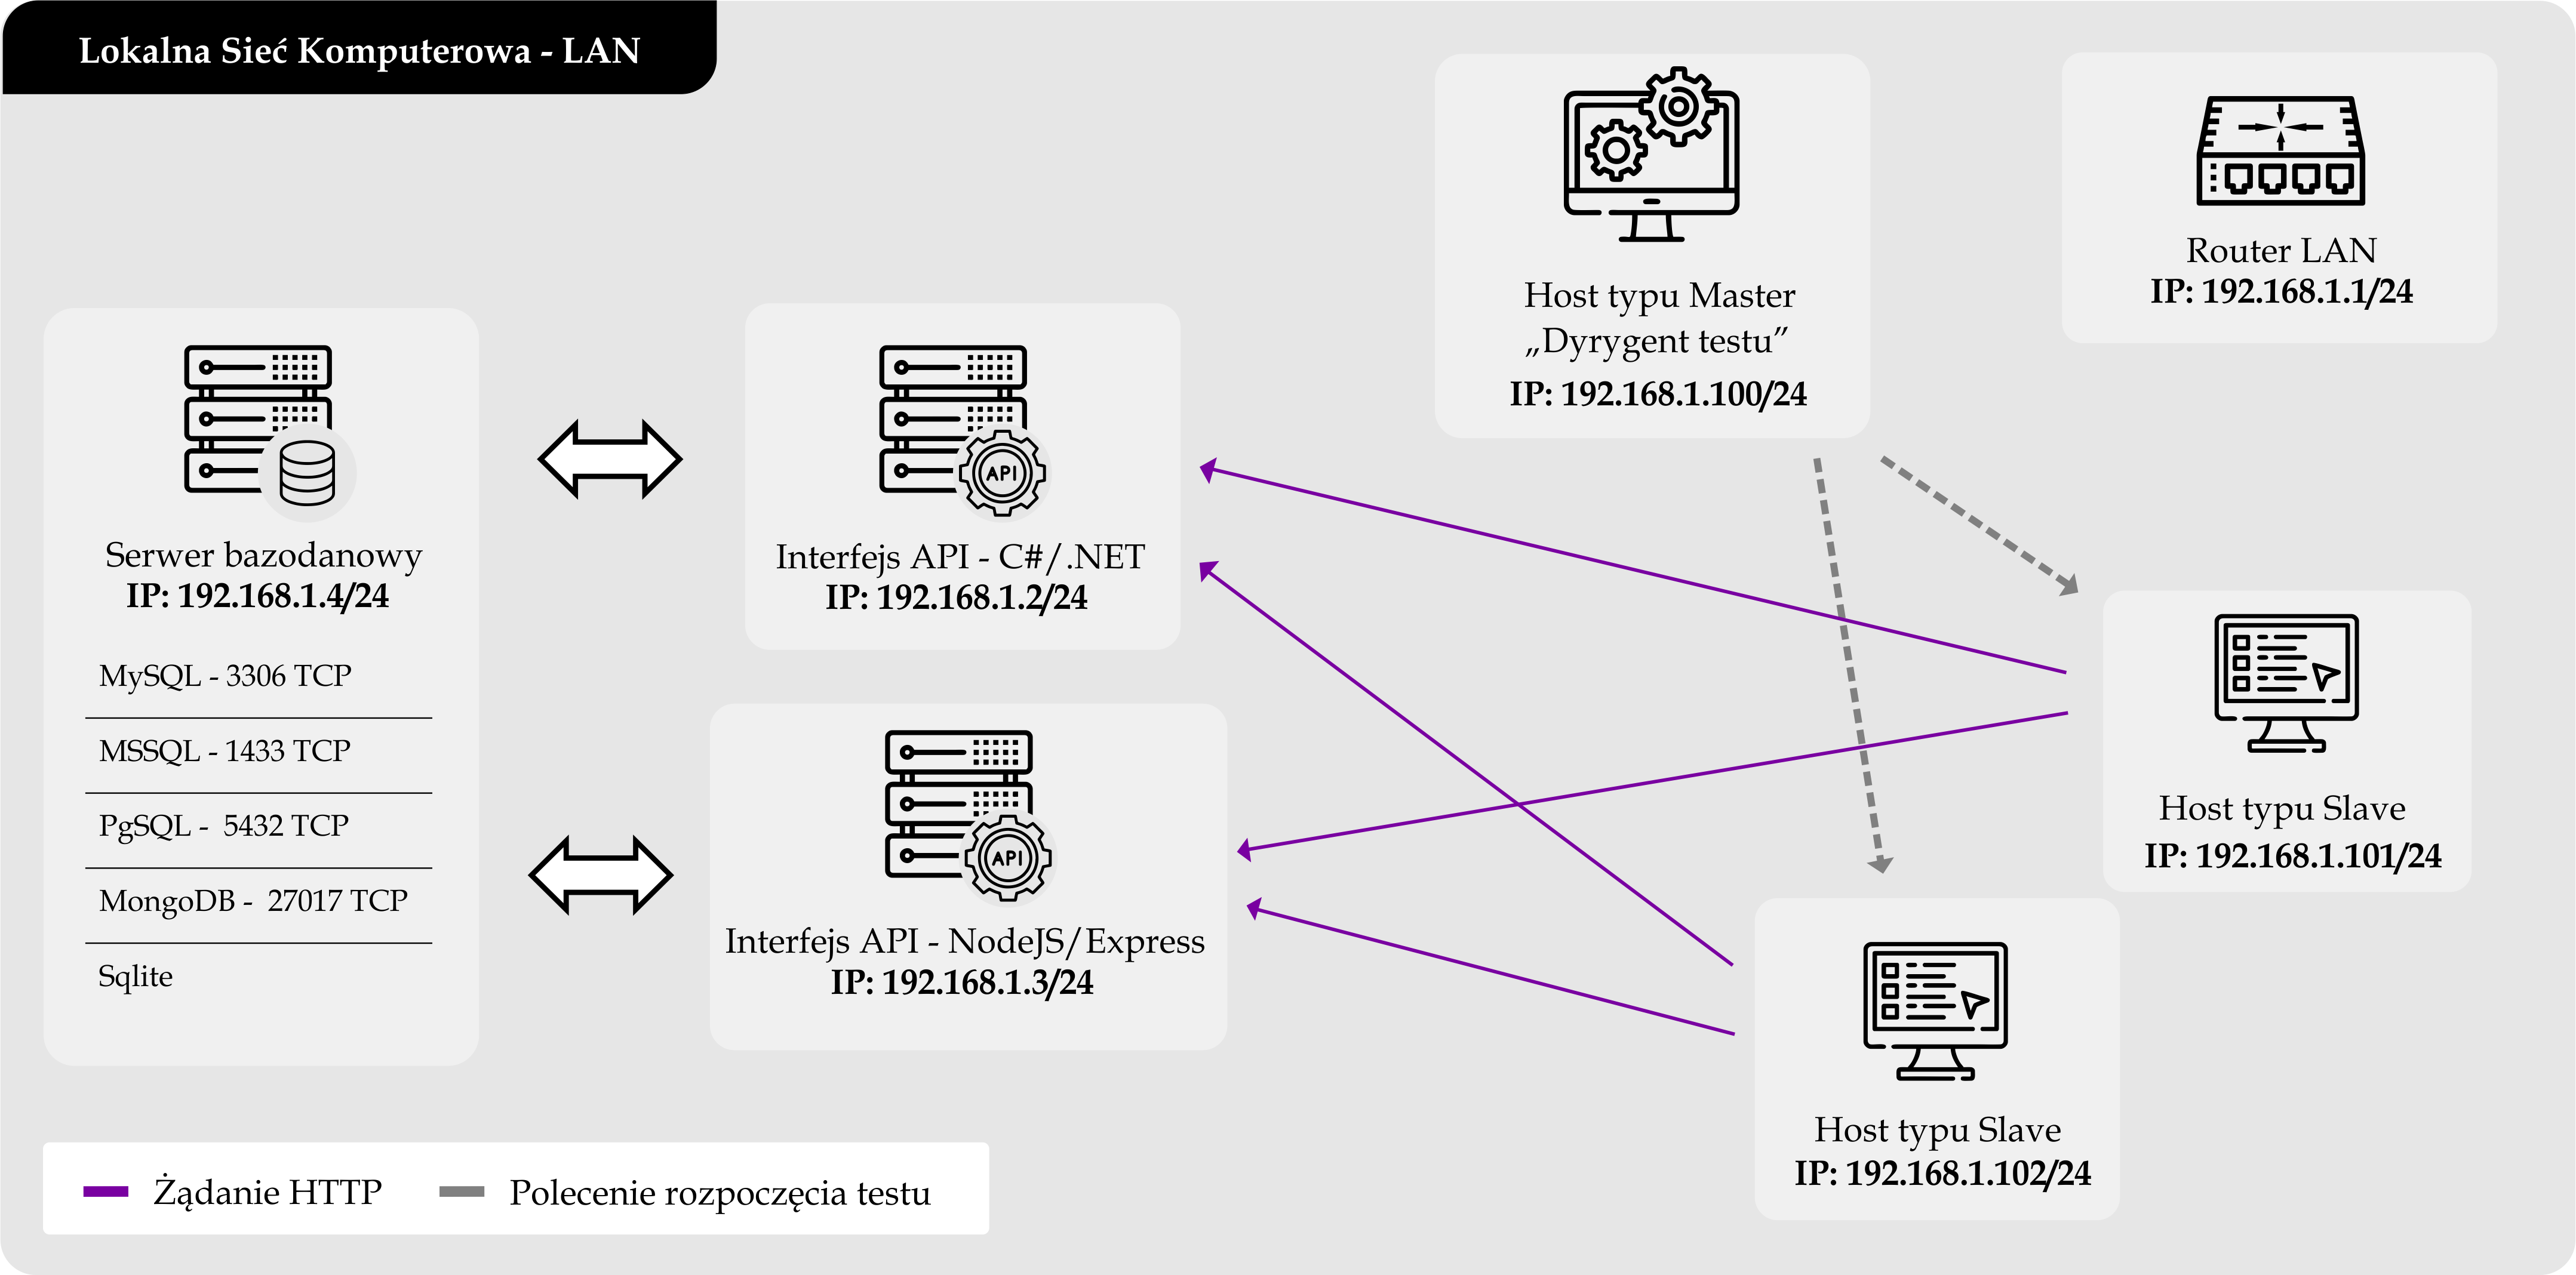
\includegraphics[width=\linewidth]{rys04/topologia-1.png}
    \caption{Konfiguracja pierwsza lokalnej topologii fizycznej środowiska badawczego}
    \label{fig:topologia-1}
\end{figure}

\subsection*{Konfiguracja druga lokalnej topologii fizycznej środowiska badawczego}
\label{sec:lokalne-srodowisko-badawcze-ver-2}
Druga topologia fizyczna środowiska badawczego, dotycząca ewaluacji w obrębie lokalnej sieci komputerowej, zbudowana została na potrzeby badań zaimplementowanych mechanizmów programowania współbieżnego, a także przechowywania odpowiedzi na żądania w ramach pamięci podręcznej.

W omawianej topologii wskazać należy dwa interfejsy programowania aplikacji, których implementacja dokonana została w porównywanych dwóch technologiach programistycznych. Obie usługi sieciowe, komunikują się z pojedyną instancją serwera bazodanowego - w przypadku badania pamięci cache, bądź też nie odwołują się do niego wcale - w przypadku badania efektywności operacji współbieżnych. Spośród urządzeń komunikacyjnych, wykorzystywanych do przeprowadzenia ewaluacji, wyróżnić należy jedno urządzenie typu Master (tzw. Dyrygent testu), a także jednego hosta typu Slave (tzw. generator żądań). Pierwszy z komputerów ma za zadanie przechowywać konfigurację wykonywanego badania, a także dostarczać komendy związane z rozpoczęciem i charakterystyką testu. Drugi host pełni rolę maszyny wytwarzającej i wysyłającej żądania protokołu hipertekstowego, zgodnie z koncepcją nakreśloną przez uzyskany plan ewaluacji. Wszystkie urządzenia znajdują się w obszarze pojedynczej, przewodowej lokalnej sieci komputerowej. Analogicznie do konfiguracji pierwszej, każde łącze przewodowe charakteryzuje się tym samym standardem oraz przepustowością.

Na ilustracji \ref{fig:topologia-2} przedstawiono schemat drugiego wariantu lokalnej topologii fizycznej środowiska badawczego.

\begin{figure}[ht]
    \centering
     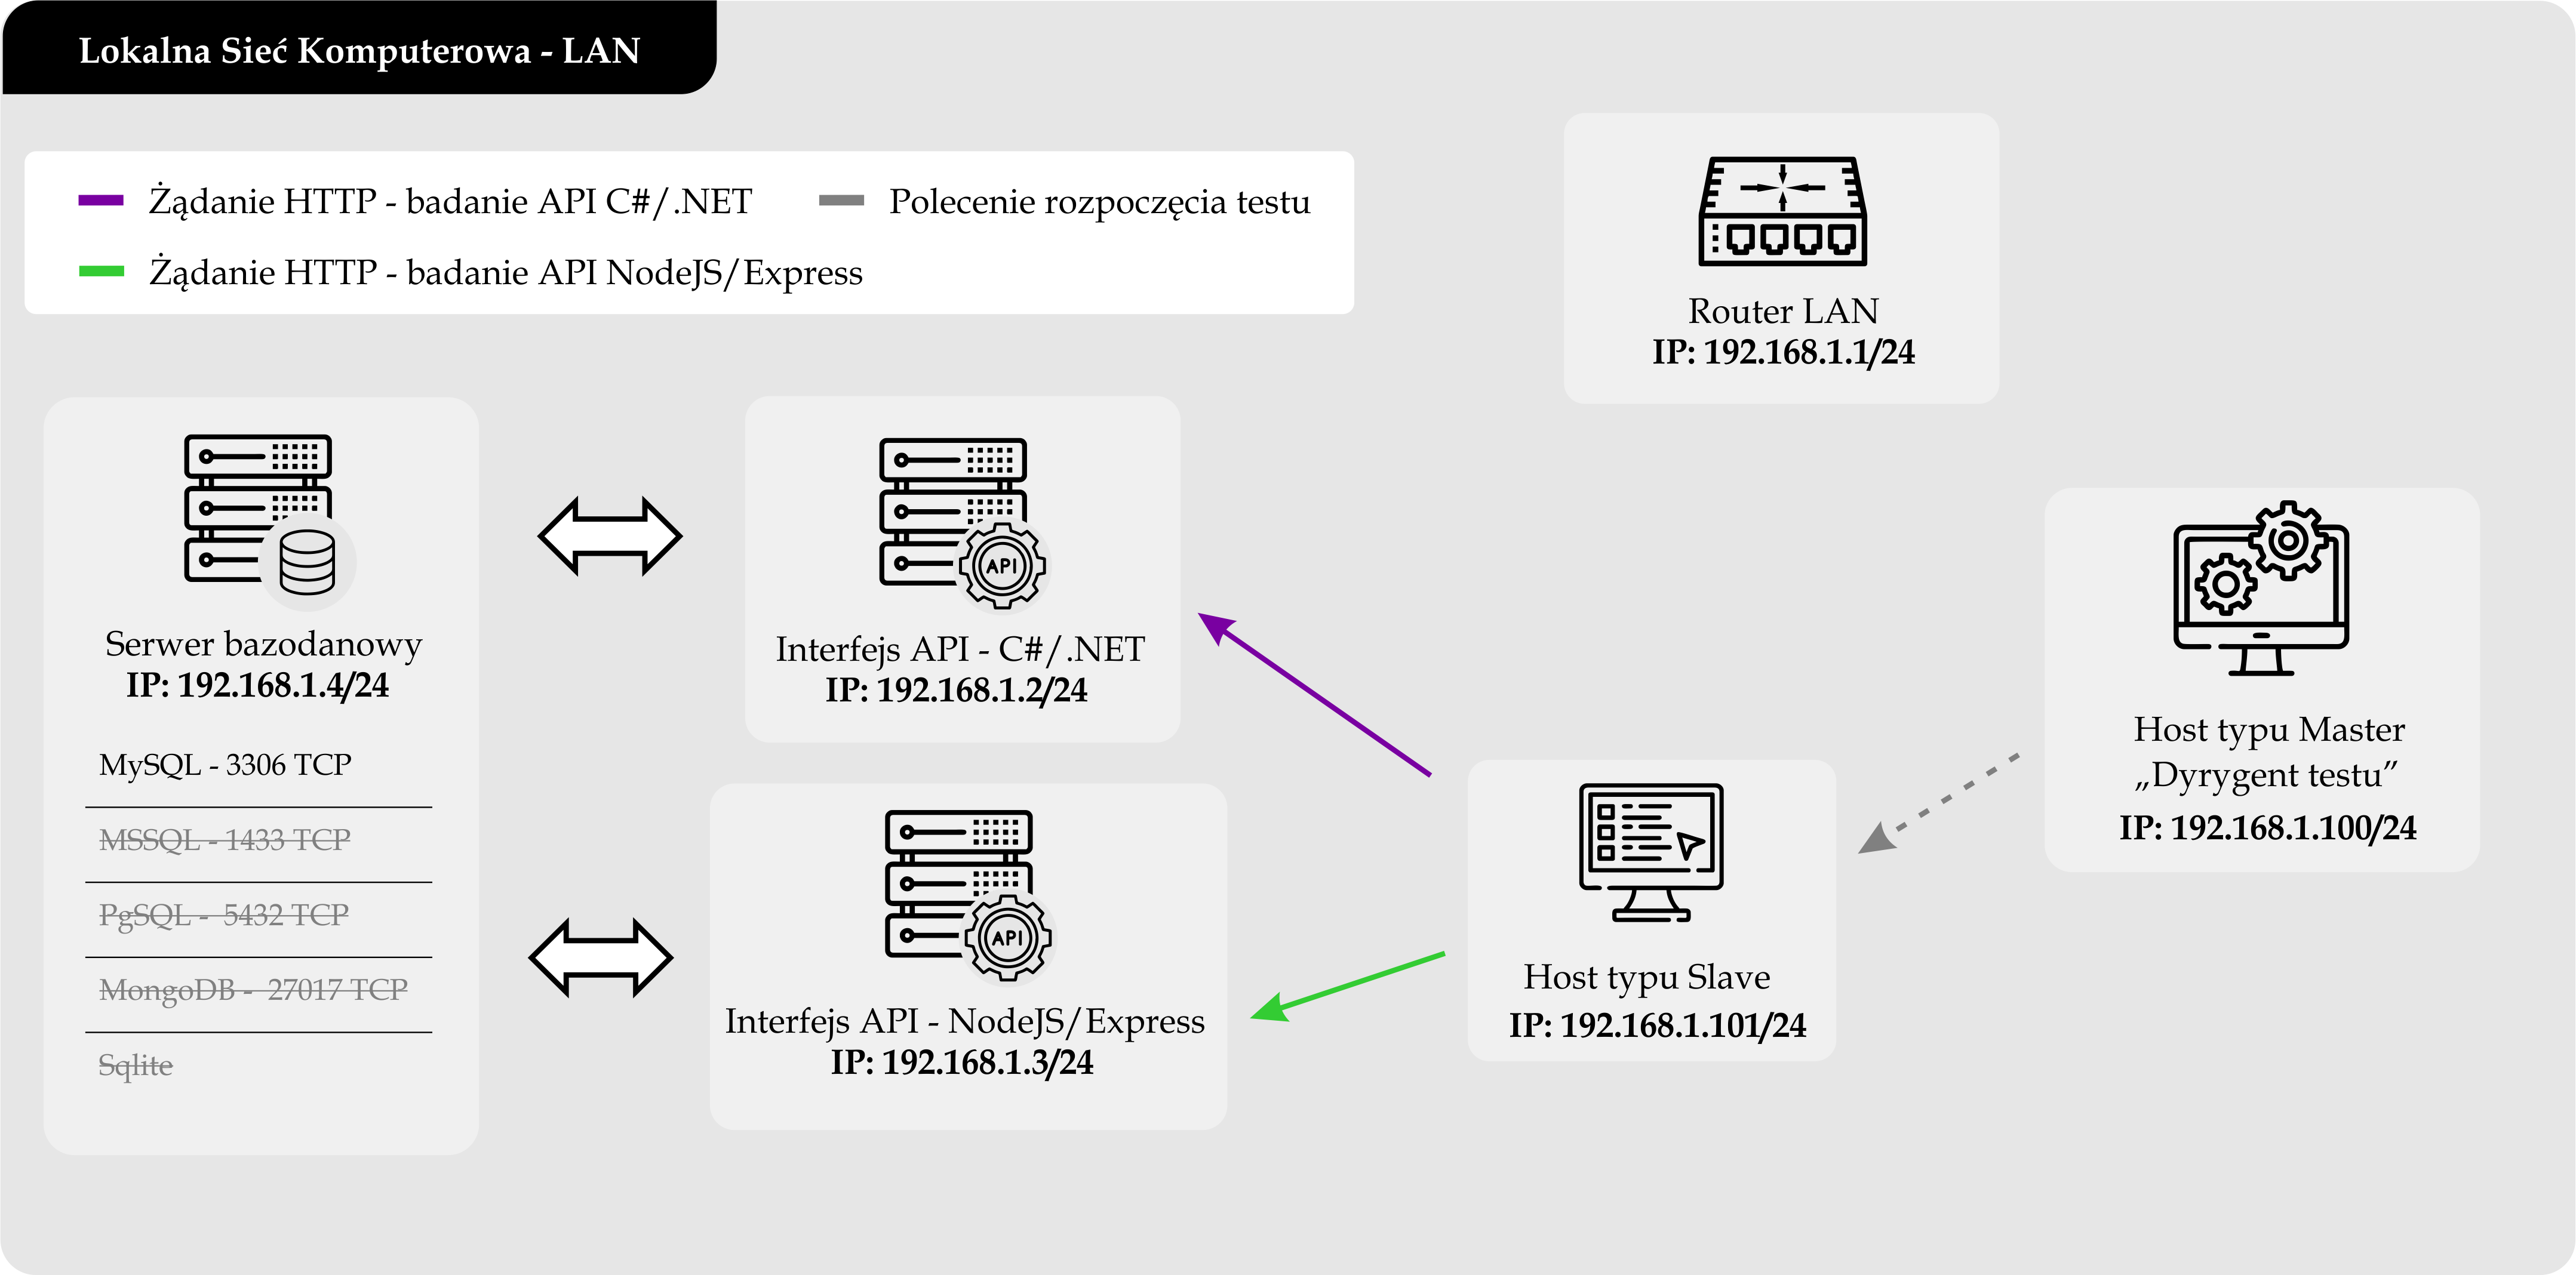
\includegraphics[width=\linewidth]{rys04/topologia-2.png}
    \caption{Konfiguracja druga lokalnej topologii fizycznej środowiska badawczego}
    \label{fig:topologia-2}
\end{figure}

\subsection*{Konfiguracja trzecia lokalnej topologii fizycznej środowiska badawczego}
\label{sec:lokalne-srodowisko-badawcze-ver-3}
Trzecia lokalna topologia fizyczna środowiska badawczego przystosowana została w celu umożliwienia realizacji badań dotyczących wydajności obsługi operacji asynchronicznych.

W schemacie tym, zauważyć można wystąpienie trzech interfejsów programowania aplikacji. Analogicznie do topologii opisanych powyżej, dwa spośród trzech API zaimplementowane są w technologiach będących przedmiotem analizy tej pracy. Trzecia usługa sieciowa, służy do udostępniania zgromadzonych w niej danych, w związku z czym posiada ona tylko i wyłącznie punkty końcowe obsługiwane z wykorzystaniem metody GET. Punkty styku ostatniego z interfejsów dostarczają funkcjonalności pobierania danych o zróżnicowanym rozmiarze.

Ponadto, zbieżnie do konfiguracji pierwszej lokalnego środowiska badawczego, wyszczególnić możemy dwa urządzenia końcowe w roli generatorów żądań, oraz jednego hosta działającego w trybie "Dyrygenta testu". Należy podkreślić, że ewaluacje dotyczące każdej z technologii, zarówno w scenariuszach badawczych wykorzystujących tę, jaki i pozostałe topologie, wykonywane są w odrębnych chwilach czasu. Implikuje to fakt, że połączenie pomiędzy hostem badającym, interfejsem badanym, a także interfejsem pomocniczym jest aktywne tylko dla aktualnie badanego rozwiązania technologicznego.

Poza interfejsami programowania aplikacji oraz urządzeniami końcowymi wskażać należy urządzenie sieciowe, jakim jest przewodowy router LAN, który łączy wszystkie elementy topologii w ramach pojedynczej sieci LAN. Standard oraz przepustowość wykorzystywanych łączy pozostaje niezmienna względem pierwszej oraz drugiej z topologii fizycznych.

Na ilustracji \ref{fig:topologia-3} przedstawiono schemat trzeciego wariantu lokalnej topologii fizycznej środowiska badawczego.

\begin{figure}[ht]
    \centering
     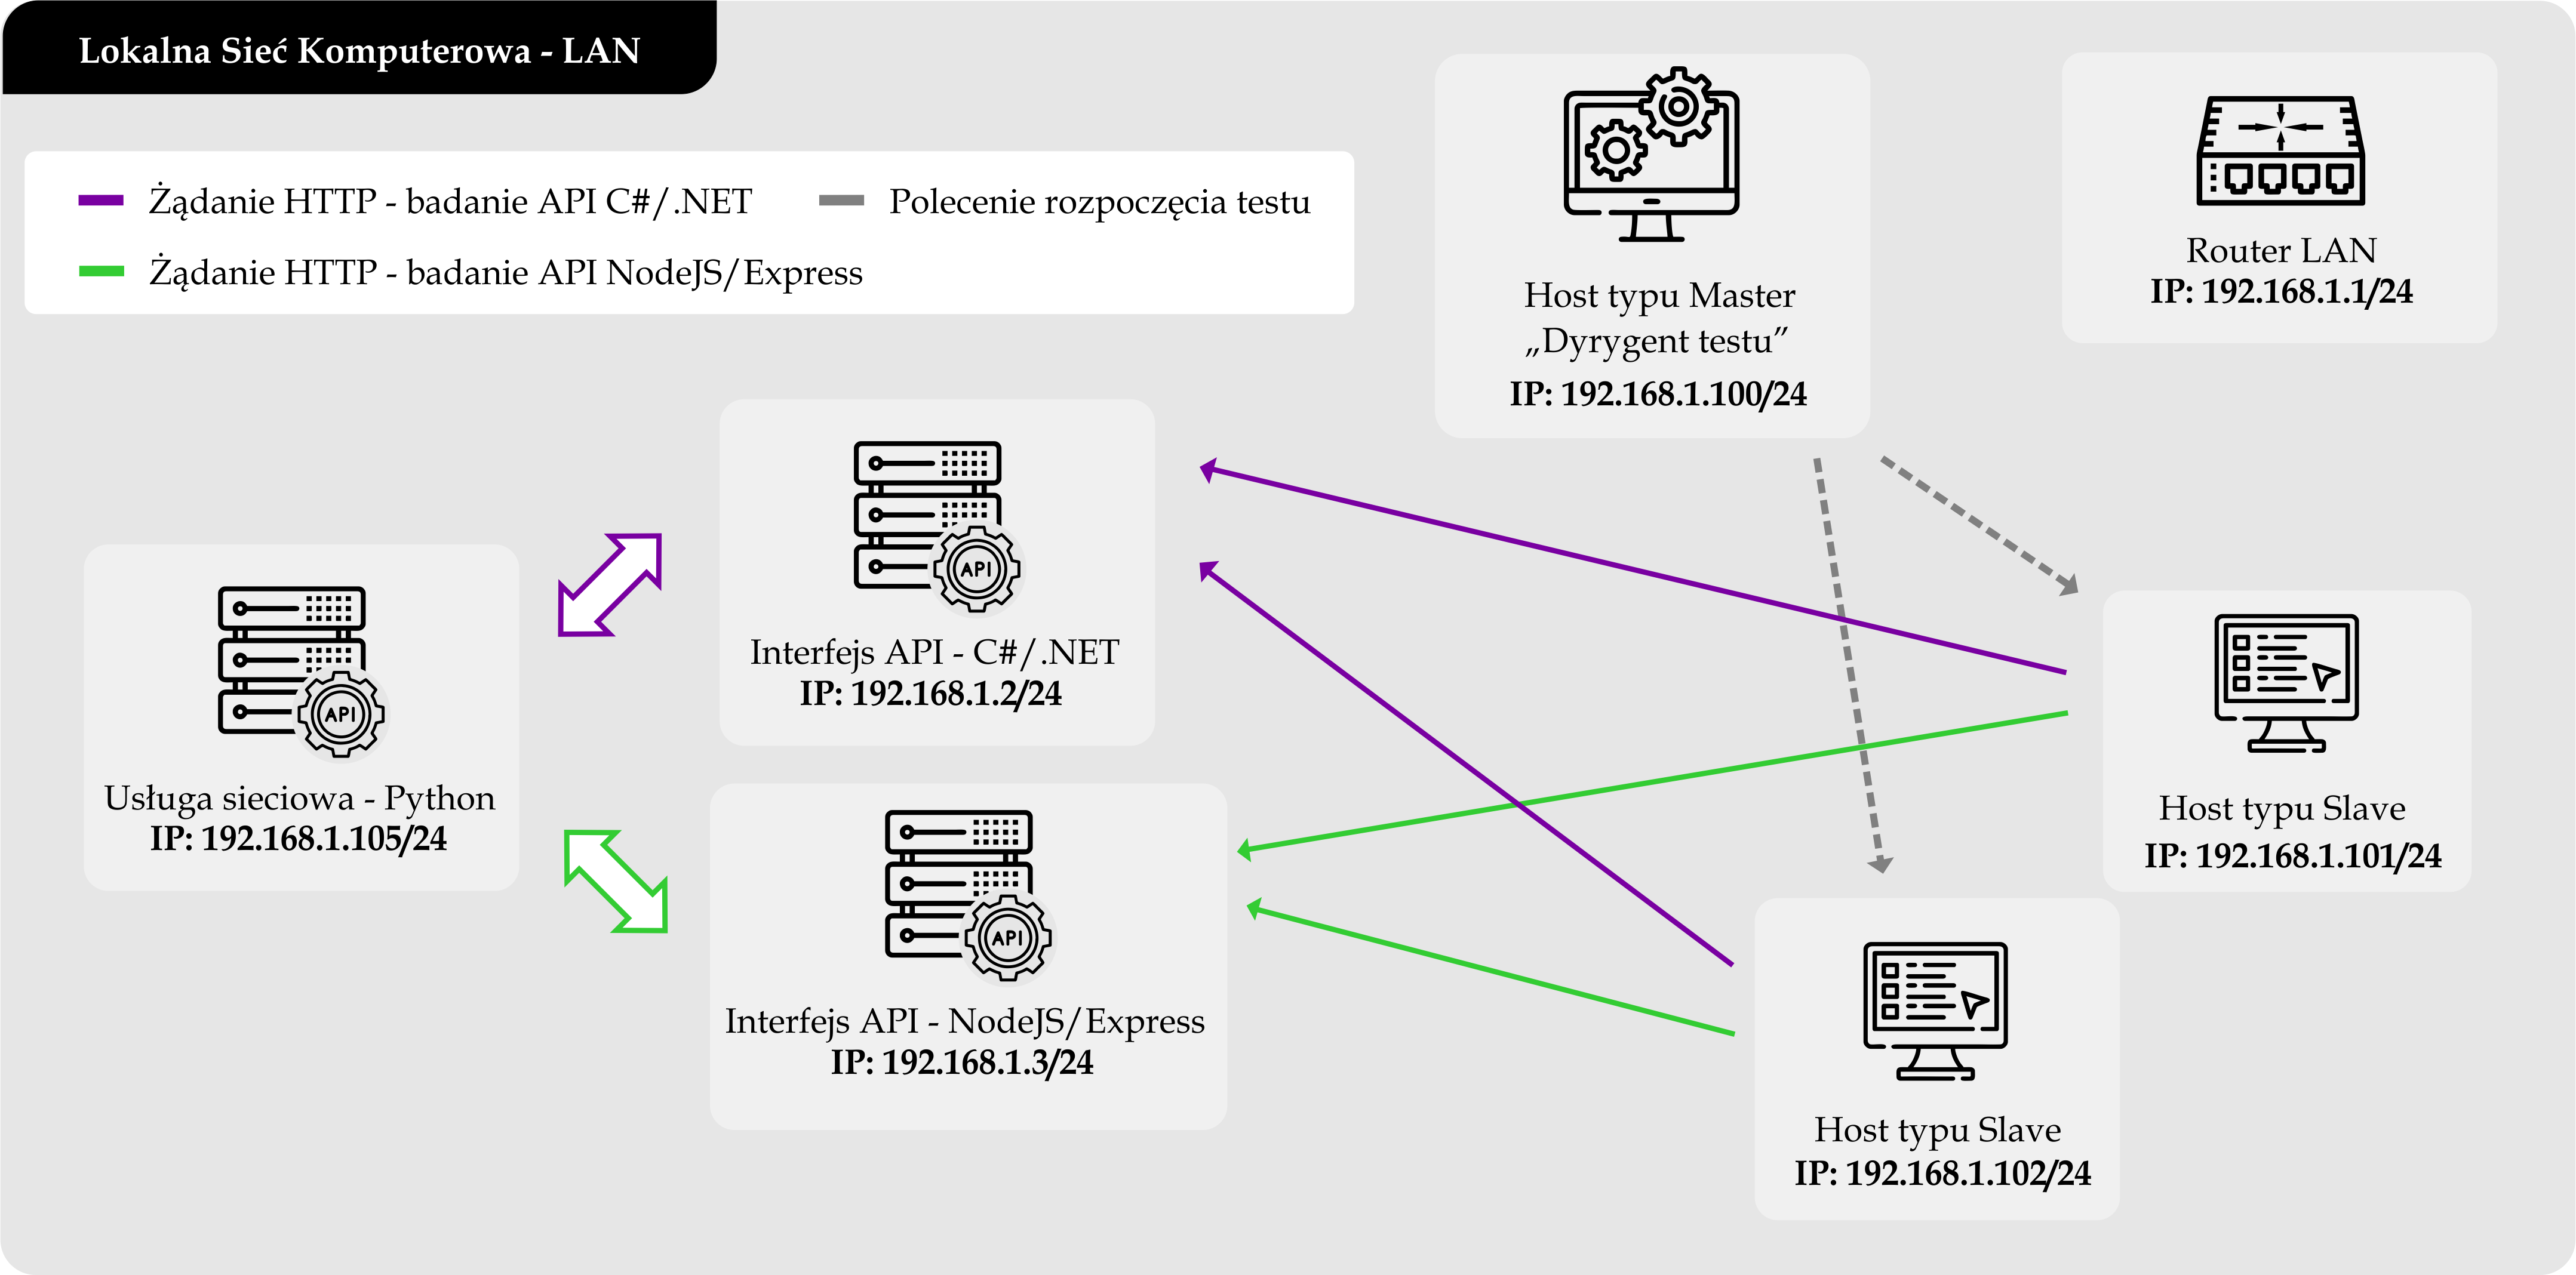
\includegraphics[width=\linewidth]{rys04/topologia-3.png}
    \caption{Konfiguracja trzecia lokalnej topologii fizycznej środowiska badawczego}
    \label{fig:topologia-3}
\end{figure}

\subsection*{Konfiguracja czwarta lokalnej topologii fizycznej środowiska badawczego}
\label{sec:lokalne-srodowisko-badawcze-ver-4}
Ostatnia z lokalnych topologii fizycznych środowiska badawczego zbudowana została w kontekście przeprowadzenia badania efektywności interfejsów programowania aplikacji w związku z zastosowaniem wzorca podziału odpowiedzialności.

Wykorzystanie tego wzorca, umożliwia separację zarówno modeli danych, jak i również fizycznych struktur bazodanowych. Dlatego też, w ramach omawianej topologii zdecydowano się na wprowadzenie dwóch oddzielnych serwerów baz danych. Serwer bazy danych wykorzystywany do zapisu implementuje operację replikacji transakcyjnej dzięki czemu, po wykonaniu zapisu do jednego źródła danych, zapisane informacje są automatycznie przenoszone do drugiej z baz. W ramach połączenia z serwerem bazodanowym wykorzystywanym do odczytu, po stronie interfejsów programowania aplikacji dokonano przystosowania modelu danych.

Poza serwerami danych, w ramach topologii wyróżnić należy dwa porównywane interfejsy programowania aplikacji, a także zbiór trzech urządzeń końcowych. Dwa spośród nich pełnią rolę generatorów żądań, natomiast trzeci host pracuje w trybie "dyrygenta testu". Wszystkie z urządzeń połączone są w obrębie lokalnej sieci komputerowej do urządzenia sieciowego którym jest router LAN.

Na ilustracji \ref{fig:topologia-5} przedstawiono schemat czwartego wariantu lokalnej topologii fizycznej środowiska badawczego.

\begin{figure}[ht]
    \centering
     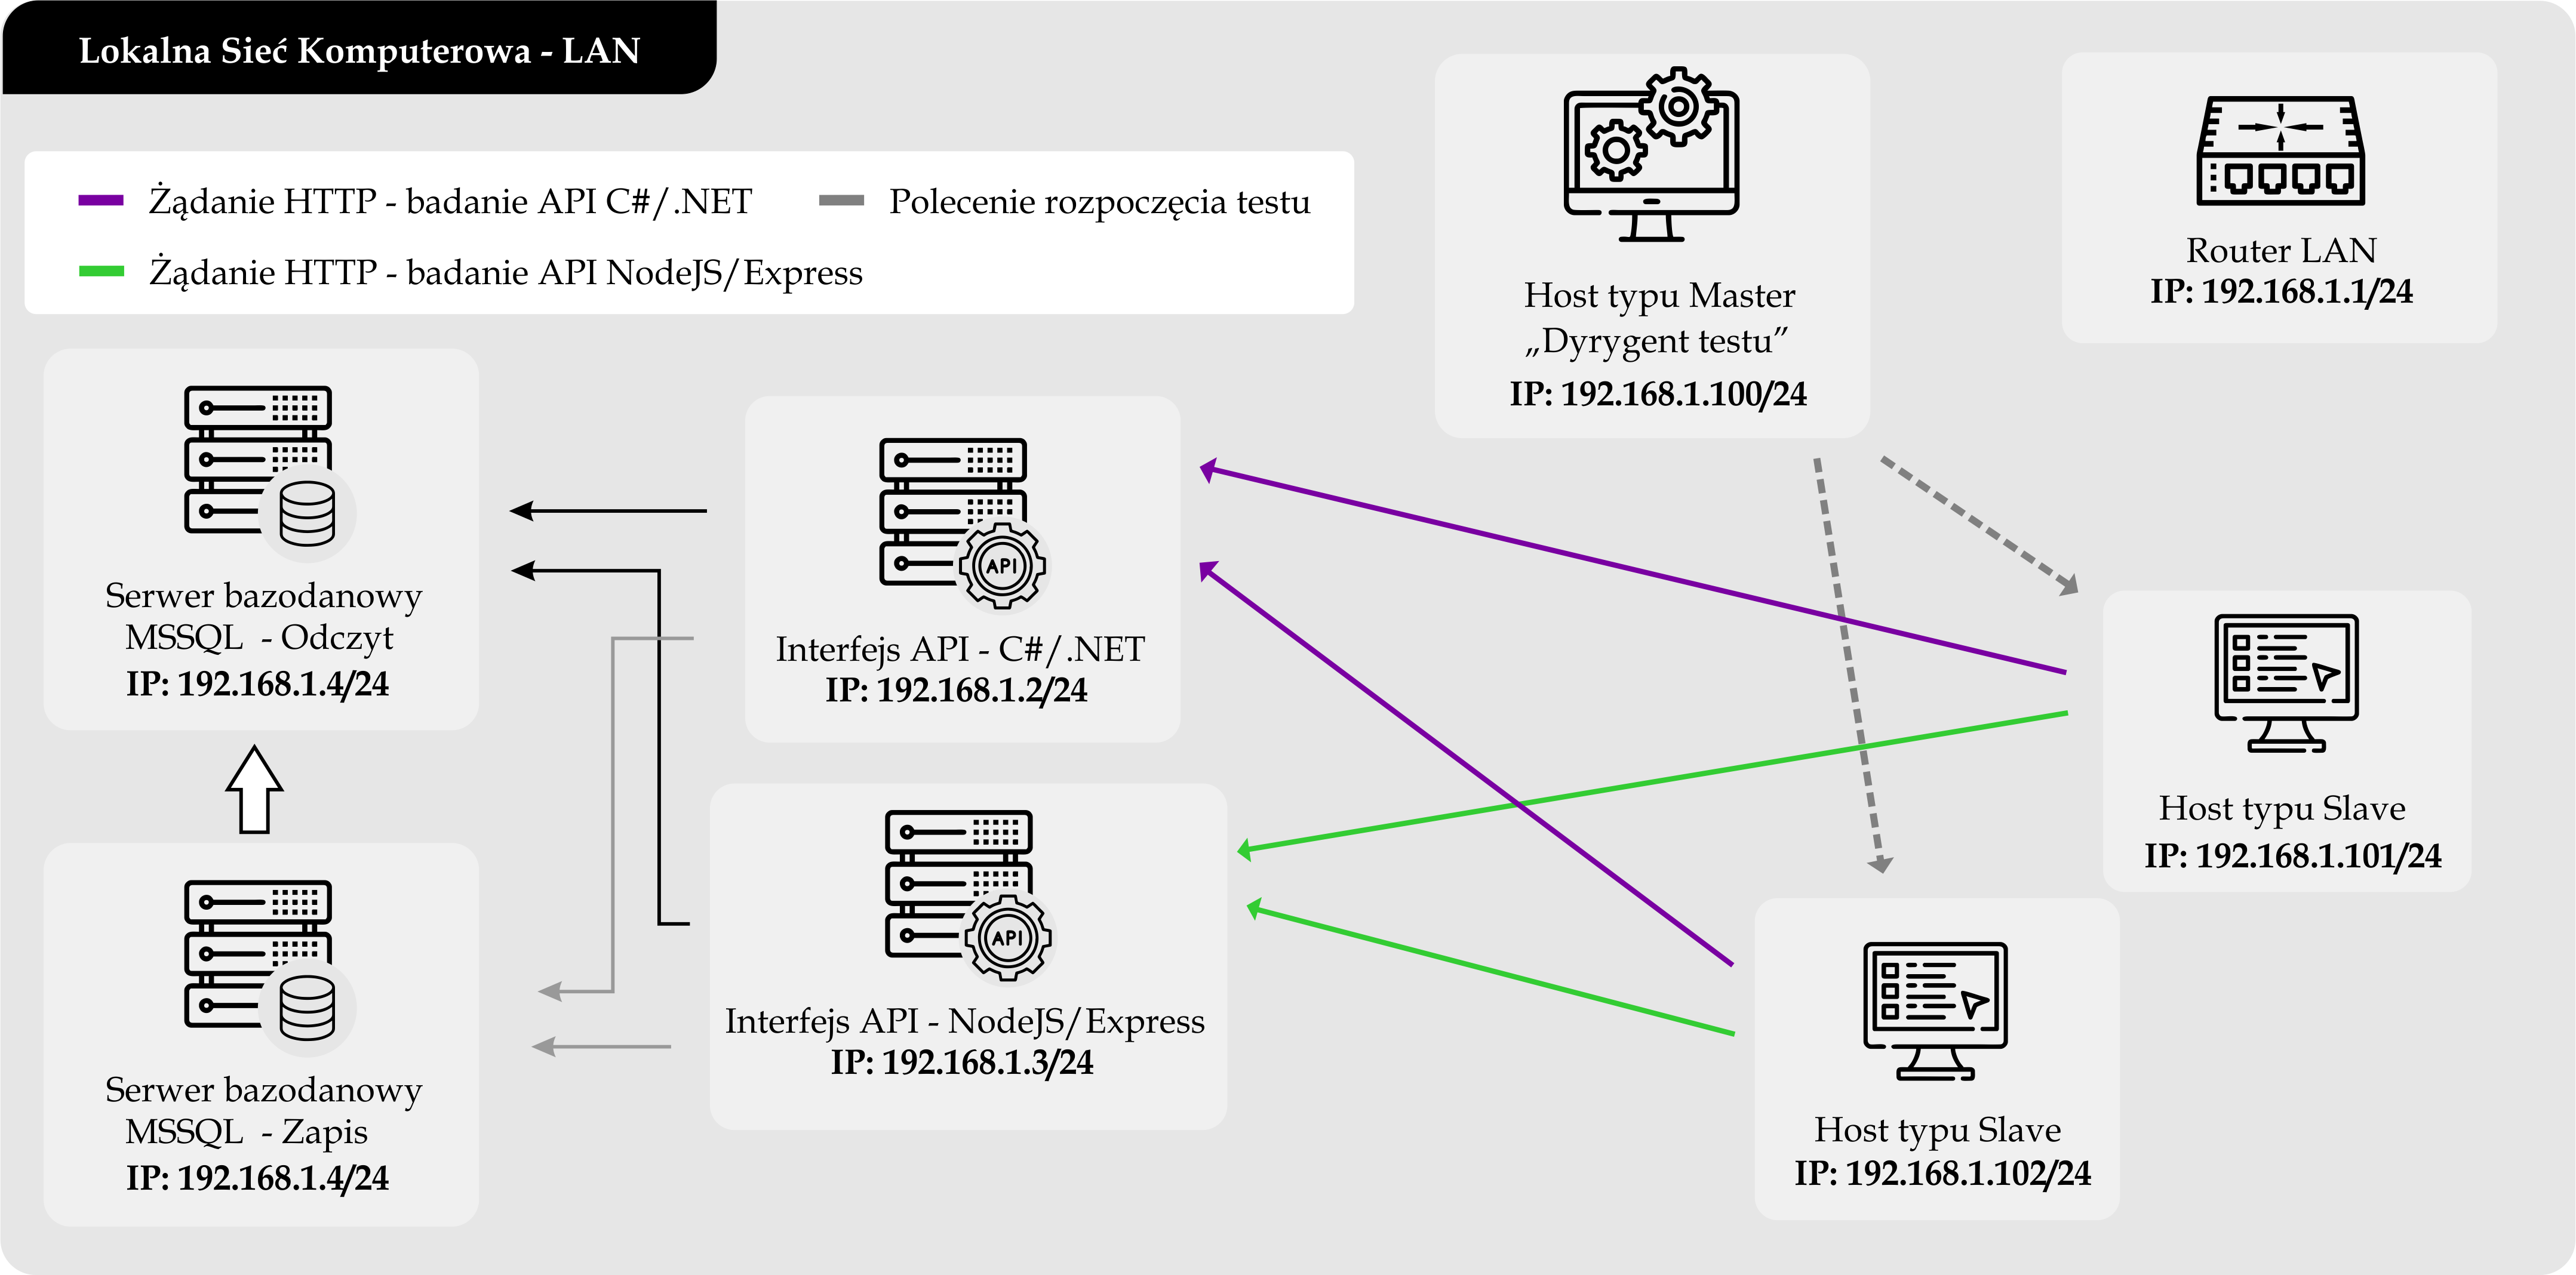
\includegraphics[width=\linewidth]{rys04/topologia-5.png}
    \caption{Konfiguracja czwarta lokalnej topologii fizycznej środowiska badawczego}
    \label{fig:topologia-5}
\end{figure}

\subsection*{Konfiguracja pierwsza rozległej topologii fizycznej środowiska badawczego}
\label{sec:rozproszone-srodowisko-badawcze-ver-1}
Konfiguracja topologii fizycznej dla rozproszonego środowiska badawczego, stworzona została w celu wykonania badań dotyczących efektywności działania interfejsów programowania aplikacji uruchamianych na odmiennych platformach chmurowych.

W tym przypadku, wyodrębnić należy dwa obszary, zawierające urządzenia w kontekście których przeprowadzana jest ewaluacja. Pierwszy obszar to lokalna sieć komputerowa, w której ulokowane zostały urządzenia końcowe odpowiedzialne za przechowywanie konfiguracji badania, a także generowanie żądań w kierunku API. W drugim obszarze zaś, nazwanym rozległą siecią komputerową uruchomione są platformy chmurowe, wewnątrz których działają interfejsy programowania aplikacji oraz serwery bazodanowe. Systemy internetowe zaimplementowane w odrębnych technologiach, przechowywane są na oddzielnych platformach chmurowych i nie są one ze sobą w żaden sposób skomunikowane. Zauważyć należy również fakt, że obie platformy chmurowe znajdują się w różnych lokalizacjach geograficznych. Stwierdzenia te, wymuszają modyfikację sposobu pozyskiwania pomiarów żądań, poprzez przeniesienie odpowiedzialności za wyliczenie czasu wykonywania operacji na interfejsy programowania aplikacji. Pomimo tego, niezbędnym jest posiadania urządzenia generującego żądania zgodnie z określoną charakterystyką. Dlatego też, wewnątrz obszaru lokalnego wskazać możemy dwa urządzenia końcowe, których rolą, podobnie do urządzeń końcowych zawartych we wszystkich poprzednich topologii fizycznych, jest generowanie żądań, oraz koordynowanie przeprowadzanego badania.

Na ilustracji \ref{fig:topologia-4} przedstawiono schemat pierwszego wariantu rozległej topologii fizycznej środowiska badawczego.

\begin{figure}[ht]
    \centering
     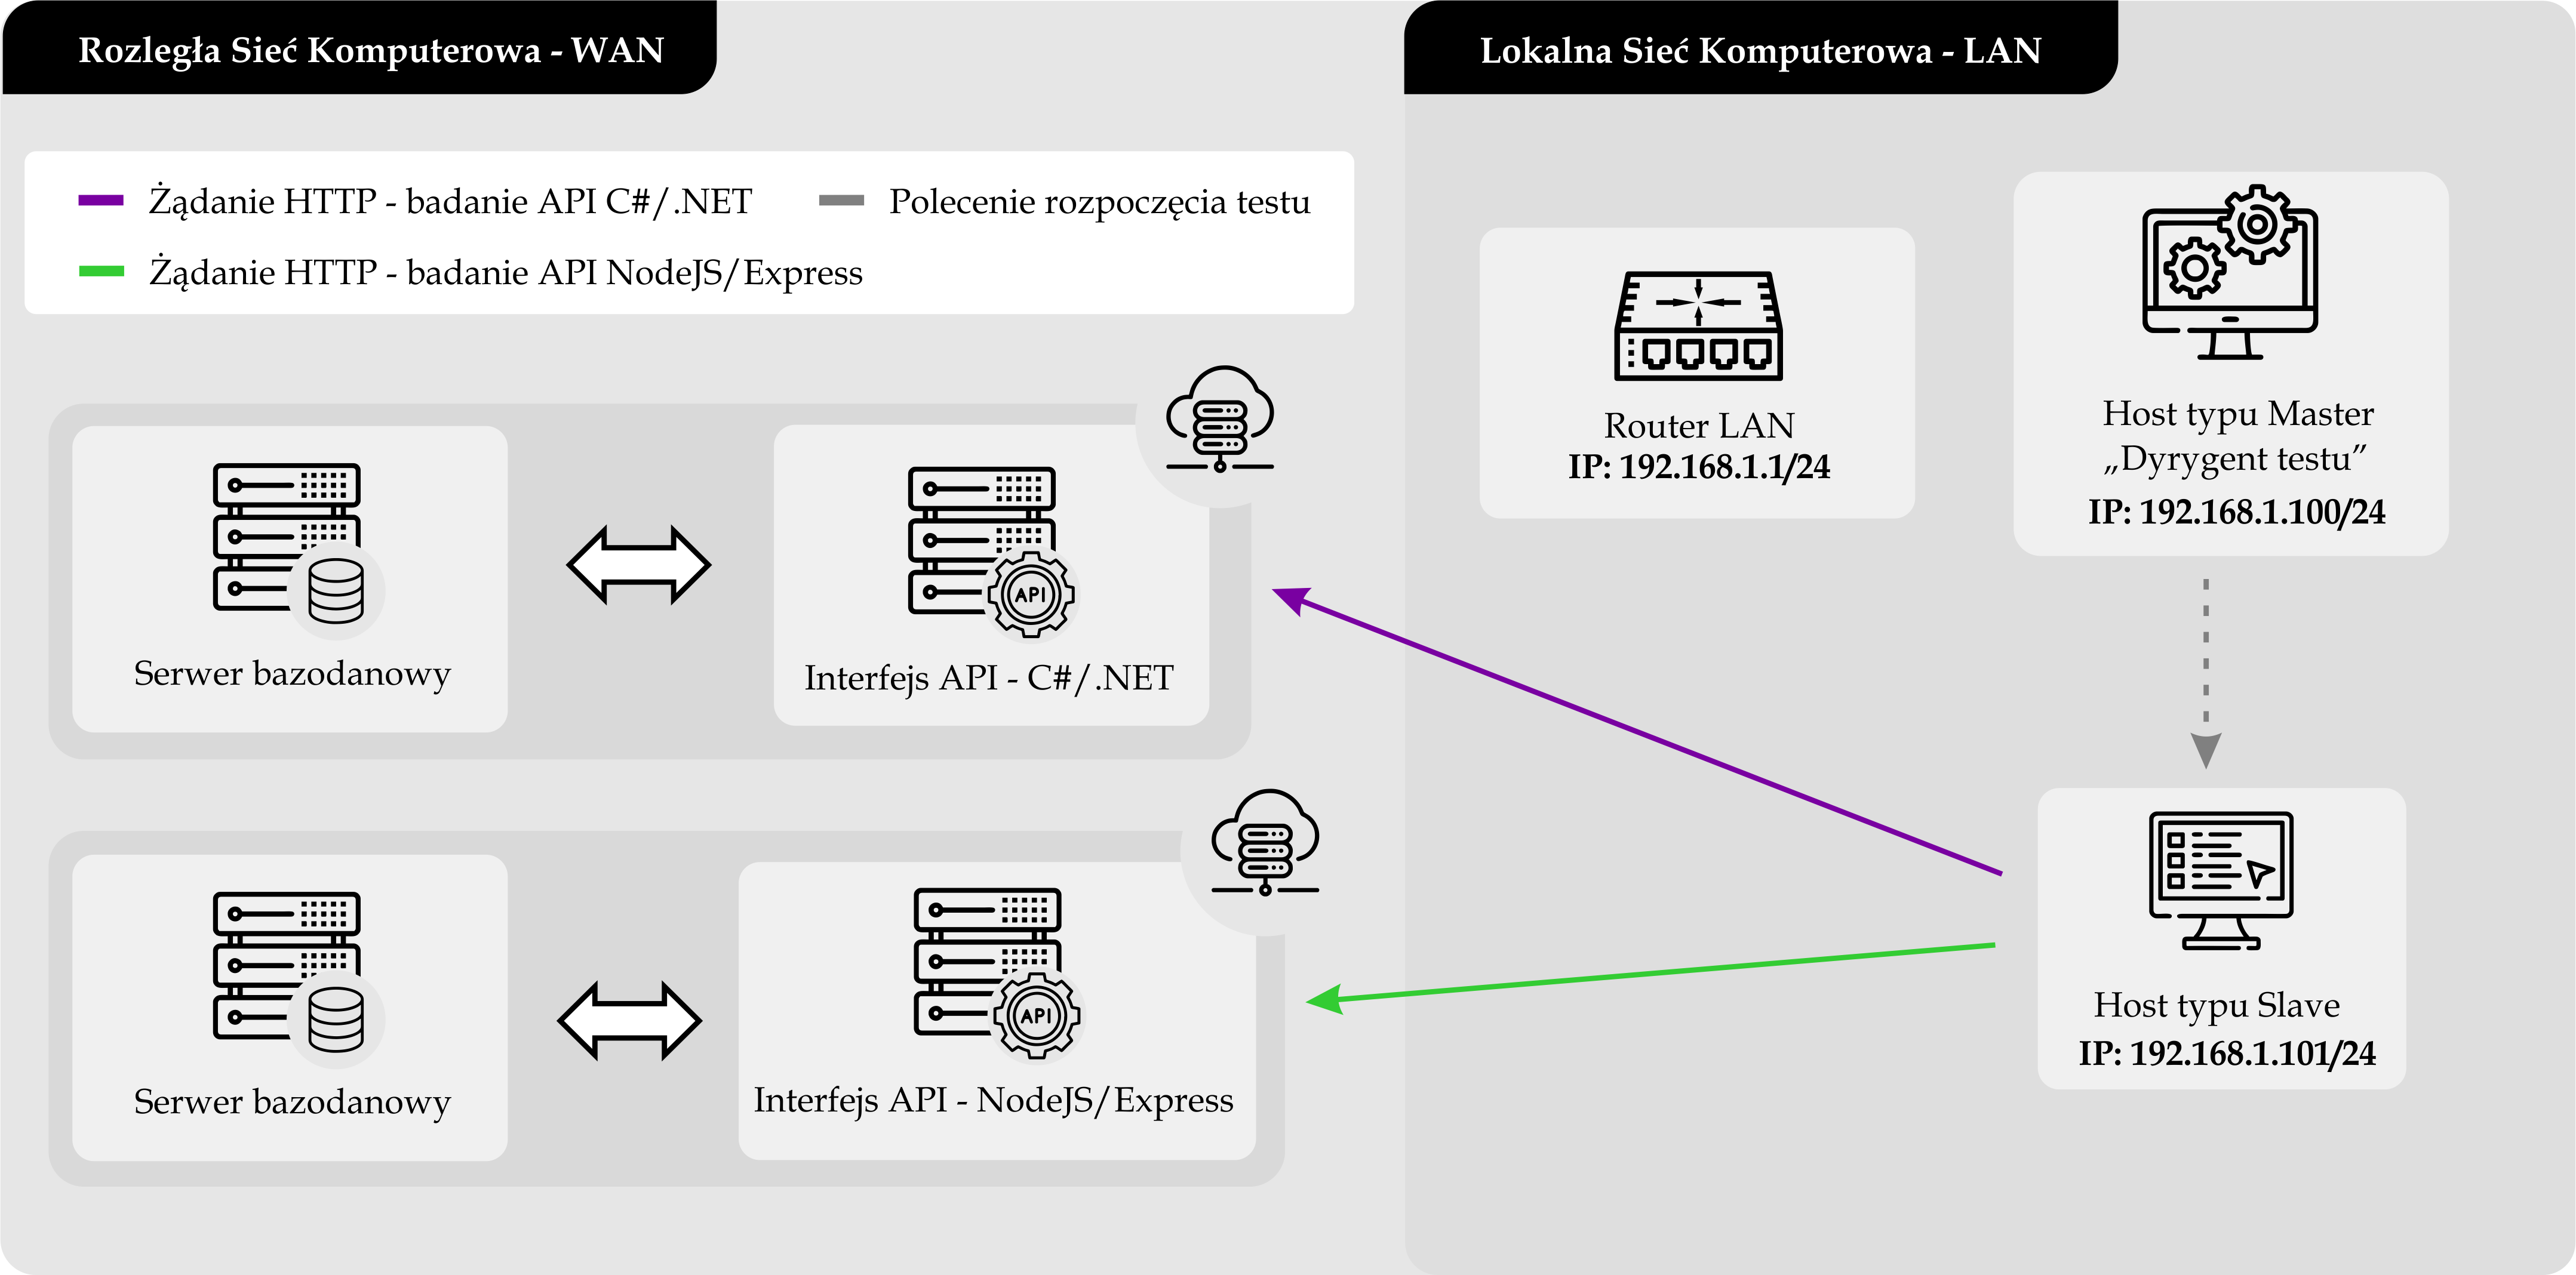
\includegraphics[width=\linewidth]{rys04/topologia-4.png}
    \caption{Konfiguracja pierwsza rozległej topologii fizycznej środowiska badawczego}
    \label{fig:topologia-4}
\end{figure}

\section{Budowa interfejsów programowania aplikacji}
\subsection*{Ogólna funkcjonalność interfejsów programowania aplikacji}
Niezależnie od rozważanej technologii, interfejsy programowania aplikacji implementowane w celu przeprowadzania badań zawartych w ramach niniejszej pracy magisterskiej, dostarczają funkcjonalności obsługi lokalu restauracyjnego. W obrębie omawianych aplikacji zdefiniować można konta użytkowników należących do jednej z pięciu ról pracowniczych. Wyróżnić możemy stanowiska: administratora systemu, zarządcy przedsiębiorstwem, kierownika sali, kucharza, a także kelnera. Użytkownicy dysponujący jedną z wymienionych ról mogą korzystać z określonego zestawu funkcjonalności, który determinowany jest poziomem uprawnień zależnych od stanowiska. Przed wywołaniem funkcjonalności systemu, każdy z użytkowników musi zostać uwierzytelniony, a także autoryzowany. Uwierzytelnienie polega na odwołaniu się do punktu końcowego logowania i podaniu swoich danych poświadczeń. Jeżeli dane poświadczeń wskazują na konkretnego użytkownika API, w odpowiedzi zwracany jest token uwierzytelniający, który musi zostać następnie dołączony do nagłówka każdego z wywoływanych żądań. Proces autoryzacji odbywa się na poziomie funkcji warstwy pośredniczącej \textit{(ang. Middleware)}, tuż przed rozpoczęciem wykonywania kodu metody klasy kontrolera.

W kontekście funkcjonalności tworzonych usług sieciowych wymienić należy:
\begin{itemize}
    \item definiowanie oraz zarządzanie strukturą lokalu restauracyjnego (zarządzanie pomieszczeniami lokalu, określanie układu stolików wewnątrz pojedynczego pomieszczenia)
    \item obsługa procesu zamównienia (zarządzanie rachunkami, daniami, statusami przetwarzania posiłków, a także dyspozycjami klientów)
    \item zarządzanie gospodarką magazynową lokalu restauracyjnego (obserwacja stanów ilościowych w kontekście produktu, obsługa danych produktu, definiowanie kategorii produktowych).
\end{itemize}

Dodatkowe funkcje systemu, nie związane z przeprowadzaniem operacji typu CRUD, takie jak wdrożenie metody wyznaczania trasy dla dostarczania zamówień, poprzez implementację algorytmu dla symetrycznego problemu komiwojażera, opisane zostały w następnych sekcjach niniejszego rozdziału.
\subsection*{Interfejs API realizujący operacje CRUD stworzony z wykorzystaniem technologii C\#/.NET}
Omawiany interfejs programowania aplikacji zaimplementowany został w języku C\#, z zastosowaniem środowiska uruchomieniowego .NET w wersji piątej. Usługa sieciowa, o której mowa w niniejszym podrozdziale, stanowi złożenie dwóch składowych. Pierwszą z nich jest program, którego zadaniem jest dostarczenie definicji oraz obsługa określonych poleceń klienta, wydanych w postaci żądań protokołu hipertekstowego. Ściśle rzecz ujmując, to właśnie ten program należy określić terminem interfejsu programowania aplikacji. Jako drugą składową natomiast, wskazać należy serwer warstwy aplikacji, pozwalający na obsługę komunikacji pomiędzy usługą sieciową a urządzeniami z zewnątrz. Serwerem wykorzystanym w ramach zaimplementowanej usługi sieciowej jest otwartoźródłowe oprogramowanie Kestrel.

W celu powiązania metod operujących na wewnętrznym modelu danych z fizycznymi strukturami bazodanowymi wykorzystano maper obiektowo-relacyjny Entity Framework Core w wersji drugiej dla relacyjnych systemów baz danych, a także narzędzie Mongoose dla nierelacyjnej bazy danych MongoDB.

Utworzone w języku C\# rozwiązanie złożone jest z pięci projektów powiązanych pomiędzy sobą zależnościami. Pierwszy z projektów zawiera klasy kontrolerów, dokumenty json globalnych właściwości usługi w określonych środowiskach, punkt startowy programu, a także klasę konfiguracji dla wszystkich definiowanych w obrębie całego rozwiązania usług. W projekcie tym, można uzyskać dostęp do struktur programistycznych, definiowanych we wszystkich pozostałych fragmentach rozwiązania.

Drugi z projektów, stworzony został z myślą przechowywania kodu źródłowego związanego z przetwarzaniem logiki biznesowej programu. Zdefiniowane zostały tu klasy serwisów, metody rozszerzeń dla typów języka, obiekt parametrów paginacji, klasy transferu danych \textit{(ang. Data Transfer Objects)}, a także prodecury generowania opowiedzi dla użytkownika. Od projektu tego, zależne są wszystkie fragmenty rozwiązania z wyłączeniem pierwszego z omawianych.

Na równorzędnym poziomie hierarchii, zdefiniowany został projekt dotyczący obsługi operacji związanych z bezpieczeństwem interfejsu API. Wyróżnić możemy tutaj klasę generatora tokenu uwierzytelniającego, a także metodę dostępu do właściwości identyfikujących użytkownika poprzez zawartość kontekstu żądania http.

Kolejnym fragmentem rozwiązania stworzonego w języku C\# jest projekt dostępu do danych. W projekcie tym, wskazać należy klasę kontekstu danych, zbiór migracji modelu danych do schematów bazodanowych, klasę propagacji danych początkowych, a także listę metod struktur repozytoriów, które pozwalają na wykonywanie bezpośrednich operacji na wykorzystywanym zbiorze informacji. Omawiany fragment, posiada zależność względem projektu logiki biznesowej.

Ostatnim projektem rozwiązania jest przestrzeń przechowywania klas modelu danych. Fragment ten, nie wprowadza zależności względem jakiegokolwiek z pozostałych projektów i pełni rolę rdzenia aplikacji. Każda z omówinionych powyżej przestrzenii kodu źródłowego posiada dostęp do elementów modelu, jednakże jakiekolwiek operacje na tych danych, wykonywane są tylko i wyłącznie z poziomie klas repozytoriów.

Na ilustracji \ref{fig:struktura-plikow-dotnet} przedstawiono strukturę obiektów wewnątrz poszczególnych fragmentów rozwiązania. Niektóre spośród elementów każdego projektu zostały pominięte na niniejszym rysunku w celu zachowania czytelności omawianej treści.

\begin{figure}[ht]
    \centering
     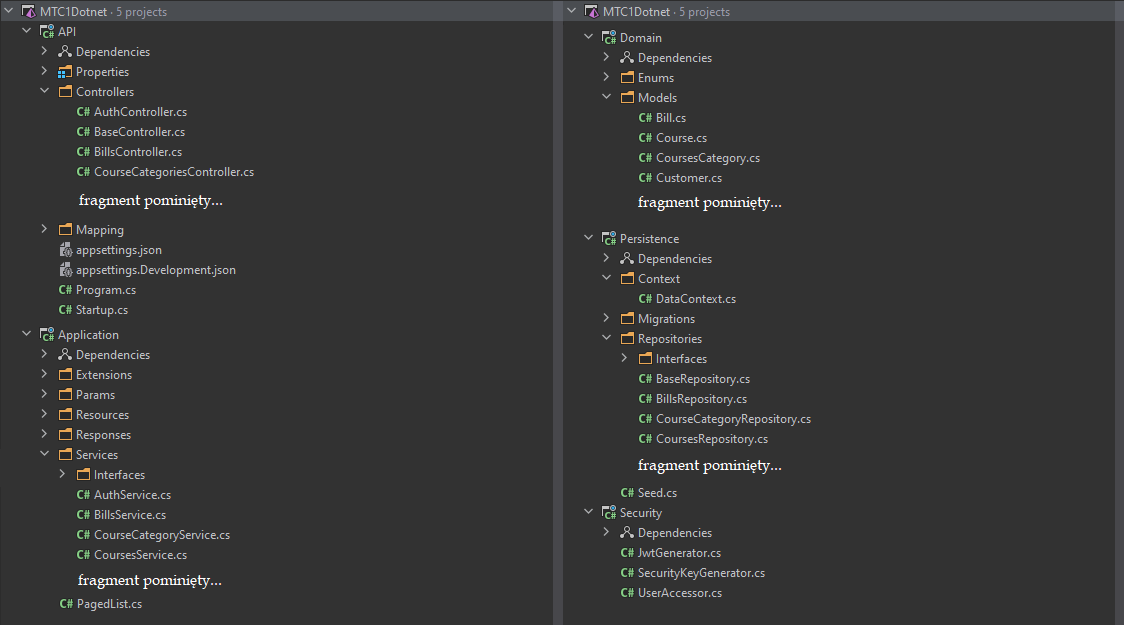
\includegraphics[width=\linewidth]{rys04/struktura-plikow-dotnet.png}
    \caption{Struktura obiektów wewnątrz rozwiązania systemu internetowego zaimplementowanego w języku C\#}
    \label{fig:struktura-plikow-dotnet}
\end{figure}
\subsection*{Interfejs API realizujący operacje CRUD stworzony z wykorzystaniem technologii NodeJS/Express}
Druga z realizacji interfejsu programowania aplikacji napisana została w języku JavaScript, zgodnym ze specyfikacją językową ECMAScript 6. Do implementacji funkcjonalności omawianej usługi sieciowej, wykorzystano bibliotekę ExpressJS w wersji czwartej, a całość oprogramowania uruchomiono na serwerze wykorzystującym natywne moduły platformy uruchomieniowej NodeJS.

W celu powiązania metod operujących na wewnętrznym modelu danych z fizycznymi strukturami bazodanowymi wykorzystano maper obiektowo-relacyjny Prisma w wersji pierwszej dla relacyjnych systemów baz danych, a także narzędzie Mongoose dla nierelacyjnej bazy danych MongoDB.

W przeciwieństwie do rozwiązania utworzonego przy wykorzystaniu technologii firmy Microsoft, schemat struktur programistycznych interfejsu programowania aplikacji opartego o JavaScript cechuje się znacząco niższym poziomem skomplikowania. Całość oprogramowania przechowywana jest w ramach pojedynczego projektu, wewnątrz którego podział struktur programistycznych ze względu na odpowiedzialności dokonany został na poziomie folderów.

Punktem startowym aplikacji, a także miejscem definicji podstawowej konfiguracji elementów usługi sieciowej jest skryptowy plik o nazwie \textit{app.js}. W pliku tym, określono wartości dla zmiennych globalnych dotyczących ścieżki podstawowej w aplikacji, czy też klucza tajnego wykorzystywanego do wyliczania tokenu uwierzytelniania. Ponadto, określono funkcje pośredniczące wykonujące się przed rozpoczęciem zadanej funkcji modułu kontrolera. Plik \textit{app.js}, zawiera także informacje dotyczące lokalizacji modułów, odpowiadających za obsługę punktów końcowych dla określonej ścieżki wywołania.

Poza plikiem startowym interfejsu programowania aplikacji wskazać należy foldery, przechowujące moduły odpowiedzialne za poprawną pracę całości aplikacji. Pierwszy z folderów o nazwie \textit{controllers}, stanowi zbiór modułów zawierających funkcje obsługujące każdy z zaimplementowanych punktów końcowych. Funkcje te, odwołują się do fragmentów oprogramowania realizujących operacje logiki biznesowej, które to fragmenty umieszczone są w folderze \textit{services}. Analogiczne odwołanie ma miejsce w kontekście modułów serwisów a funkcji operujących na danych. Funkcje te, znaleźć można w folderze \textit{repositories}. Ponadto, wyróżnić należy katalog \textit{errors}, przechowujący kod źródłowy dotyczący przetwarzania błędów dla każdej z logicznych warstw interfejsu, katalog \textit{helpers} w ramach którego zdefiniowane zostały funkcje pomocnicze, a także folder \textit{prisma}, zawierający w sobie pliki migracji oraz dokument definicji schematu modelu danych.

Na ilustracji \ref{fig:struktura-plikow-nodejs} przedstawiono strukturę obiektów wewnątrz poszczególnych fragmentów rozwiązania. Niektóre spośród elementów każdego projektu zostały pominięte na niniejszym rysunku w celu zachowania czytelności omawianej treści.

\begin{figure}[ht]
    \centering
     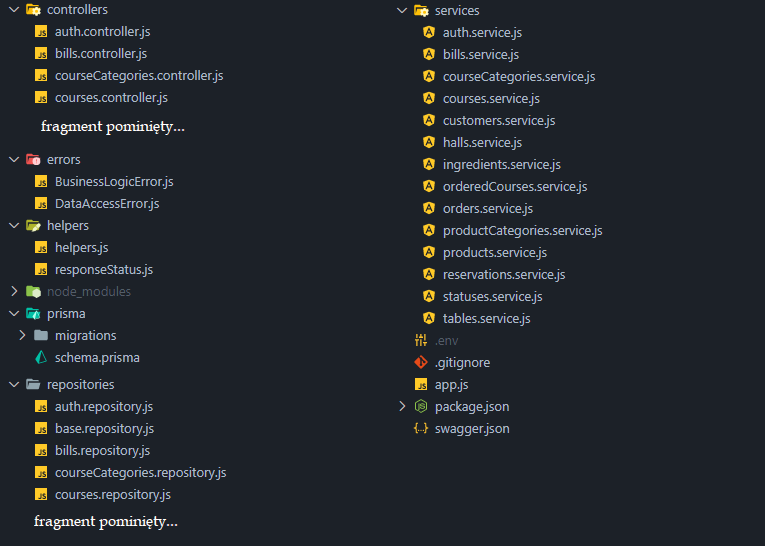
\includegraphics[width=\linewidth]{rys04/struktura-plikow-nodejs.png}
    \caption{Struktura obiektów wewnątrz rozwiązania systemu internetowego zaimplementowanego w języku JavaScript}
    \label{fig:struktura-plikow-nodejs}
\end{figure}

\subsection*{Algorytm metaheurystyczny dla symetrycznego problemu komiwojażera dostępny z poziomu punktu końcowego}
\subsection*{Mechanizm obsługi pamięci podręcznej z uwzględnieniem częstotliwości wywoływania punktów końcowych}
\subsection*{Implementacja wzorca projektowego CQRS z uwzględnieniem replikacji danych pomiędzy dwoma źródłami}
\section{Konfiguracja generycznych oraz dedykowanych platform chmurowych}
\section{Konfiguracja narzędzia do realizacji badań}


